% !Mode:: "TeX:UTF-8"
%!TEX program  = xelatex

\documentclass{cumcmthesis}
%\documentclass[withoutpreface,bwprint]{cumcmthesis} %去掉封面与编号页

\usepackage{url}
\usepackage{booktabs}

\usepackage[colorlinks,
             linkcolor=blue,       %%修改此处为你想要的颜色
            anchorcolor=blue,  %%修改此处为你想要的颜色
            citecolor=blue,        %%修改此处为你想要的颜色,例如修改blue为red
             ]{hyperref}
             
%\usepackage[compress]{cite}
\title{ }
\tihao{A}
\baominghao{4321}
\schoolname{西北工业大学}
\membera{于欣雨20.49}
\memberb{杨雨民}
\memberc{陈城钰}
\supervisor{贾万涛}
\yearinput{2019}
\monthinput{09}
\dayinput{15}

\begin{document}

 \maketitle
 \begin{abstract}
我们猜测APP的定价策略是出于对任务的等级首先进行划分,再通过对任务标价进行微调,最终才会出现集中落在以5为间隔的任务标价附近。我们认为,这一现象出现主要是因为由于会员的分布也是以市中心为中心逐渐向外扩散,我们猜想会员的密度为定价的主要因素之一。通过对四个城市对比会员数量与任务标价相关系数为-0.97,说明会员数量与人物标价线性负相关,验证了我们之前的猜想。同时,根据附件二的信息,我们发现信誉值与任务限额对定价也有一定的影响,APP为了吸引更多的新用户和培养忠实用户,一般它的定价算法会选择给新会员较高的定价,以提高会员的忠实度。我们还发现完成率与该城市GDP相关性为-0.78,这说明,任务完成率还与任务当地的经济情况有关系。而四个市的经济情况非常不同,四个城市定价策略的参数应该不同。

针对问题二,计算出距离各个会员的距离,从中选出100个最近的会员,取出这100个会员的距离,信誉值和任务限额的平均值作为这个任务的影响因素。然后对每一个成功完成的任务,计算出如上数据,利用多元线性回归得到回归方程。最后根据回归方程计算未完成的任务的期望定价,进行修正。我们的以平均距离、平均信誉值和平均限额为变量的多元线性拟合取得了比较满意的结果。但是我们同时发现我们的模型对郊区的高价任务标价有着较高的拟合度,而对市区的定价大多都高于原价。

针对问题三,我们通过修改问题二中定价模型,从而导出适用于含任务包的任务定价方案。 首先,在考虑会员预定限额的基础上,确定了以标价和距离为影响因子的接单概率模型。通过加入信誉值对完成概率的影响,进而建立了完成概率的模型。受到物流配送区域划分方法的启发,建立了基于点密度的任务聚类模型对任 务进行打包处理。进而类比问题二,建立了含任务包的目标规划模型,确定最优定价, 并得出此定价下的任务完成概率。与问题二中任务完成率、标价总额进行对比,结果表 明,将任务打包后任务完成率提高。其中打包后的任务理论完成率为:0.8059,有显著提升。

针对新项目任务分布高度集中的特点,需要结合实际,对任务包内任务 个数进行限制。基于任务个数上限,对问题三打包方案进行了改进,运用改进后的打包 方案对任务打包后,通过建立含任务包的目标规划定价模型,确定了每项任务的定价。 结果分析表明,在此方案下任务完成率为:0.5042。



\keywords{多元线性回归\quad  聚类分析\quad   非线性优化模型\quad  }
\end{abstract}




%目录
\tableofcontents
\newpage
\section{问题重述}

高压油管的压力控制是燃油发动机的效率的重要保障。在燃油进入和喷出高压油管时,其间歇性的工作过程会导致高压油管内压力的变化,从而使喷出的燃油量出现偏差,从而影响发动机的工作效率,因此如何设置泵油策略显得尤为重要。燃油经由高压油泵进入油管,再由喷油嘴喷出。

\textbf{问题1:}给定高压油管的结构数据、压力初始值及油泵、喷油嘴的工作机制,要求设置合理的单向阀开启时长,使得管内的压力在工作期间稳定在100Mpa。若需要使管内压力由100MPa增至150MPa,且分别规定调整时间为2s、5s和10s,需分别给出单向阀开启时长的策略。给定数据为:油管内腔长度为500mm,内直径为10mm,供油入口小孔直径为1.4mm;单向阀每打开一次后就要关闭10ms,喷油器每秒工作10次,每次工作时喷油时间为2.4ms。

\textbf{问题2:}在问题1的基础上,将油泵及喷油嘴的工作原理细化,要求求出高压油泵中凸轮的角速度,使油管内压力稳定在100MPa。进入高压油管的燃油来自高压油泵的柱塞腔出口,喷油由喷油嘴的针阀控制。在高压柱塞油泵的压油过程中,凸轮通过驱动柱塞上下运动来压缩柱塞腔内的燃油。当柱塞腔内的压力大于高压油管内的压力时,单向阀开启,燃油进入。其中柱塞腔内直径为5mm,柱塞运动到上止点时,腔内容积为20mm3;运动到下止点时,低压燃油充满腔内,其压力为0.5MPa。喷油器喷嘴结构如图所示,燃油在针阀上升时流出油管,且已知针阀升程与时间的关系。其中,针阀直径为2.5mm,密封座圆锥半角为9度,最下端喷孔直径为1.4mm,喷油器工作次数、高压油管尺寸和初始压力同问题1。



\textbf{问题3:}在问题2的基础上,再增加一个喷油规律相同的喷油嘴,请调整并给出喷油和供油策略。为更好地控制高压油管的压力,现计划在D处安装一个单向减压阀,其出口为直径为1.4mm的圆,打开后高压油管内的燃油可以在压力下回流到外部低压油路中,使得高压油管内燃油的压力减小。请给出高压油泵和减压阀的控制方案。

\section{模型的假设}
\begin{itemize}
\item 根据题目要求,由于管道内燃油压力变化量与密度变化量成正比,假设管道内液体为可压缩液体,且管道内部各处压力分布均一,即:压力仅随时间变化,而不随位置变化。

\item 本文忽略燃油进入和喷射系统在喷射过程中的其他影响因素,如针阀的运动惯性、喷嘴油腔容积的变化、油泵进回油孔的节油现象、针阀与导向套间及柱塞与柱塞套间的泄露等。

\item 本文忽略加热和传热过程以及热力对热油管道的影响。
\end{itemize}

\section{符号说明}

\begin{center}
	\begin{tabular}{cc}
		\toprule[1.5pt]
		\makebox[0.3\textwidth][c]{符号}	& \makebox[0.4\textwidth][c]{意义} \\
		\hline
	 $E$ & 弹性模量 \\
	$P$ & 高压油管内的压力 \\  
	$\rho$ & 燃油密度 \\ 
	$C$ & 流量系数 \\
	$A$ & 小孔的面积 \\
	\bottomrule[1.5pt]
	\end{tabular}
\end{center}

\section{问题分析}
\subsection{问题1}
针对问题1,需要设置单向阀每次开启的时长使得高压油管内的压力在燃油规律进出时稳定在100MPa左右。为此,我们设置一个函数表达式以衡量这一目标,即求出管内平均压力P关于单向阀开启时长$t_{1}$的微分表达式。通过观察目标值是否接近100MPa,对变量$t_{1}$不断进行迭代,从而得到最佳结果。

首先,根据题目所给信息及实际情况可知,燃油的密度随着压力而变化。通过附件3所给数据,可通过拟合得出弹性模量与压力P之间的三次表达式,即可通过弹性模量表示密度。又由题可得,燃油的压力变化量与密度变化量成正比,且比例系数为$E/\rho$,因此由上一步可求得比例系数,从而得出压力变化量与密度变化量之间的关系表达式。

接着,通过质量守恒定律建立模型,得出管内燃油质量在进行流入、流出操作后的变化量,又因为管内燃油总体积不变,因此可得油罐内密度的变化量。管内燃油质量的变化量与进入流量$Q_{in}$与流出流量$Q_{out}$相关。$Q_{in}$与$Q_{out}$在工作时的流量大小表达式已由题可知,此时设置一个开关函数$s(t)$与两个出入口工作时的流量大小相乘(开关函数由工作时长$t_{1}$进行条件约束),以考虑油泵与喷油嘴的间歇性工作状态。最终将$Q_{in}$,$Q_{out}$分别与进出时的燃油密度相乘并相减,则可得到高压油管内燃油质量的变化量。最终得到质量变化量与密度变化量之间的关系,即密度变化量与单向阀工作时长之间的关系式。yuxinyu

将上述关系式带入压力变化量与密度变化量之间的关系表达式,得到压力变化量与单向阀工作时长之间的关系,即管内平均压力P关于单向阀开启时长$t_{1}$的微分表达式。之后即可通过观察目标值是否接近100MPa,对变量$t_{1}$不断进行迭代,从而得到最佳结果。

\begin{figure}[!htp]
	\centering
	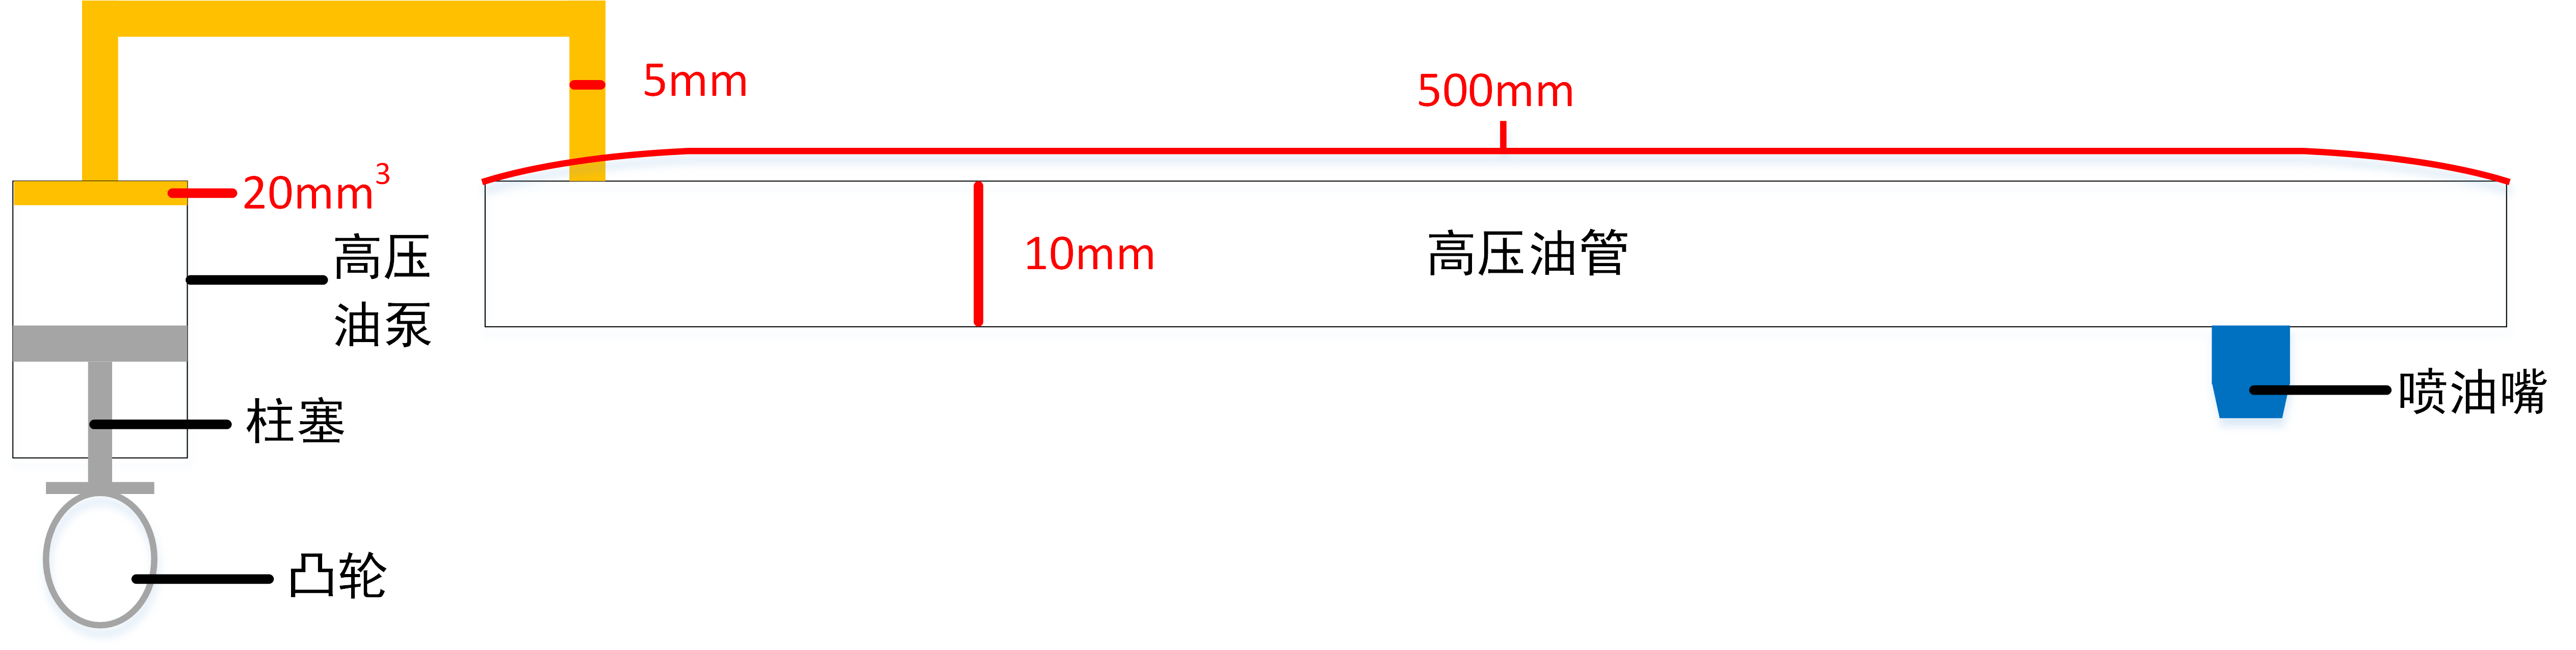
\includegraphics[width=.8\textwidth]{gyyg.png}
	\caption{高压油管实际工作示意图}
	\label{1}
\end{figure}

问题1:问题1题目已知高压油管的结构数据、压力初始值及油泵、喷油嘴的工作机制,要求设置合理的单向阀每次开启时长以尽可能稳定高压油管内压力。
\begin{figure}[!htp]
	\centering
	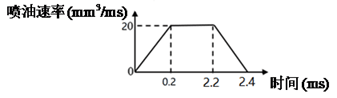
\includegraphics[width=.4\textwidth]{pysl.png}
	\caption{喷油速率示意图}
	\label{2}
\end{figure}

问题2:问题2要求需要我们对任务定价规律进行分析,

问题3:问题3要求此处要求修改问题 2 的定价模型,将多个位置比较集中的任务联合在 一起打包发布并优化问题 2 中的新模型,并分析打包对模型的影响。 

\section{模型的建立与解决}
\subsection{问题1:单向阀开启控制模型}
问题1要求在满足题目给出的喷油嘴工作情况下,设置单向阀每次开启时长,使高压油管内压力尽可能稳定。本小组首先利用三次多项式拟合确定弹性模量$E$随压力$P$变化公式,并结合压力变化量$P$与密度变化量$d\rho$的关系,获得密度与压强的关系。随后,结合质量守恒定律建立单向阀开启控制模型,获得最终的单向阀开启控制方案。
\subsubsection{密度与压强关系的确定}
根据附件3中提供的弹性模量与压力之间的关系可知,假设弹性模量$E$与压力$P$有关,其关系为:
	\begin{equation}
		E=E(P)
	\end{equation}
利用三次多项式拟合得:
\begin{equation}
\frac{1}{E(P)}=-1.9222 \times 10^{-12}P^{3}+1.7574\times 10^{-9}P^{2}-2.0512\times 10^{-6}P+6.4998\times 10^{-4}
\end{equation}
\begin{figure}[!htp]
	\centering
	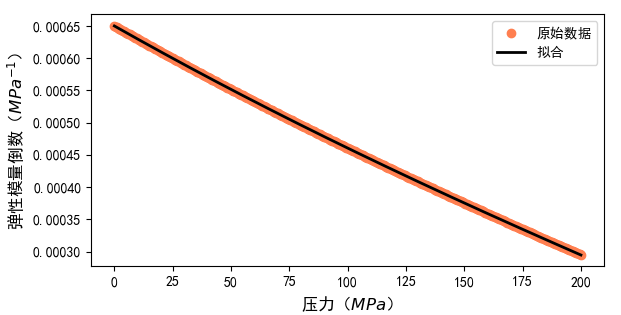
\includegraphics[width=.8\textwidth]{pmf.png}
	\caption{三次多项式拟合压力与弹性模量倒数的关系}
	\label{3}
\end{figure}
此时显著性水平$R^{2}=1.0000$,拟合精度较高,$P$和$E$的单位均为$MPa$。

已知燃油的压力变化量$dP$与密度变化量$d\rho$成正比,其比例系数为$\frac{E}{\rho}$,得:
\begin{equation}
dp=\frac{E(P)}{\rho}d\rho
\end{equation}
两边同时积分得:
\begin{equation}
	\int{\frac{dP}{E(P)}}=\int{\frac{d\rho}{\rho}}
\end{equation}
结合$\rho(100)=0.85$,得到密度与压力之间的关系:
\begin{equation}
\rho=exp(-4.8056\times 10^{-13}P^{4}+3.8579\times 10^{-10}P^{3}-1.0256\times 10^{-6}P^{2}+6.4998\times 10^{-4}P-0.2178)
\end{equation}

\begin{figure}[!htbp]
	\centering
	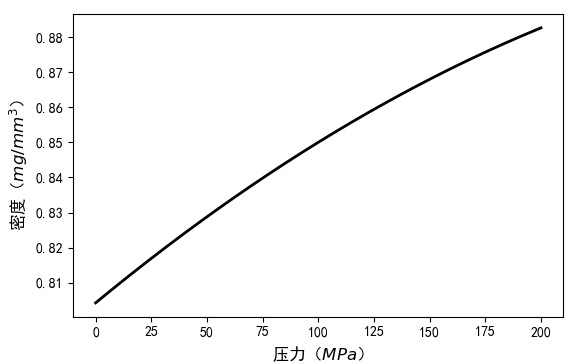
\includegraphics[width=.45\textwidth]{pd.png}
	\caption{密度与压力关系}\label{4}
\end{figure}

\subsubsection{质量守恒定律}	
根据已知得到高压油泵进油流量$Q_{in}$和喷油嘴出油流量$Q_{out}$公式如下:
\begin{equation}
\begin{cases}
Q_{in}=CA\sqrt{\frac{2\Delta P_{1}}{\rho}}S_{1}(t)\\
Q_{out}=Q_{out}(t)
\end{cases}
\end{equation}
其中,
\begin{equation}
s_{1}(t)=
\begin{cases}
1,\qquad n(t_{1}+10)< t_{1} \leq (n+1)t_{1}+10n,\qquad n=0,1,2,3,......\\
0,\qquad (n+1)t_{1}+10n < t_{1} \leq (n+1)(t_{1}+10),\qquad n=0,1,2,3,......
\end{cases}
\end{equation}
\begin{equation}
Q_{out}(t)=
\begin{cases}
100t,\qquad 100n<t\leq 100n+0.2\\
20, \qquad 100n+0.2<t\leq 100n+2.2\\
100(2.4-t), \qquad 100n+2.2<t\leq 100n+2.4\\
0, \qquad 100n+2.4<t\leq 100(n+1)
\end{cases}
\end{equation}
高压油管内部体积保持恒定,根据质量守恒定律,得:
	\begin{equation}
	dm=(\rho_{1} Q_{in}-\rho_{2}Q_{out})dt
	\end{equation}
	\begin{equation}
dP=\frac{E}{\rho}\frac{dm}{V}
\end{equation}
利用数值积分最终获得压力随时间的变化关系:
\begin{equation}
P=P(t)
\end{equation}


	
	
\subsubsection{单向阀开启控制方案}
	
	






\section{模型的改进}
本文在分析任务分配的过程中,未考虑每个会员开始预定时间的差异。实际上,由 于任务的分配原则,预定开始时间晚的会员在预定任务时会受到之前预定此任务会员的 影响,即在实际过程中,会员预定各任务的概率是随时间变化的。

在会员预定任务时,发现已经预定此任务的会员人数较大,就会导致该会员预定此 任务的概率变小,且该会员会更倾向于选择已经预定人数较少的任务。该现象表明,会 员预定某个任务的概率与其预定时刻任务点已有预定的会员数具有负相关性。 

因此,我们需要加入会员开始预定时间对众包任务的分配过程进行仿真模拟。

\section{模型的优缺点}
\subsection{模型的优点}
\begin{enumerate}
\item 本文能有效量化标价及距离对任务完成情况的影响。 
\item 在设计定价方案时,对个体行为进行了分析,使得出的标价与任务完成情况之 间的关系更加合理
\item 本文能有效量化标价及距离对任务完成情况的影响。 
\item 在设计定价方案时,对个体行为进行了分析,使得出的标价与任务完成情况之 间的关系更加合理
\end{enumerate}
\subsection{模型的缺点}
\begin{enumerate}
\item 在分析定价规律时,仅从宏观角度考虑影响定价的因素,还需从任务点区域的 经济水平、交通状况等角度综合考虑对任务定价的影响。 
\item 问题二中求解多目标规划模型的算法复杂度较高
\item 本文对时间对任务的影响并没有很好的考虑,进一步用时间修正模型难度较大。
\end{enumerate}

%参考文献


\bibliography{exam}
\bibliographystyle{is-unsrt}

%\begin{thebibliography}{99}%宽度9
% \bibitem{bib:one} 韩中庚,数学建模方法及其应用,北京:高等教育出版社,2009。 
% \bibitem{bib:two}姜启源,谢金星,叶俊,数学模型,北京:高等教育出版社,2003。 
% \bibitem{bib:three}龚纯,王正林,精通 MATLAB 最优化计算,北京:电子工业出版社,2012。 
% \bibitem{bib:four}卓金武,李必文,魏永生,秦健,MATLAB 在数学建模中的应用,北京:北京 航空航天大学出版社,2014。
%\end{thebibliography}

\newpage
%附录
\appendix
\section{主程序--matlab 源程序}
\begin{lstlisting}[language=matlab]
function [dist,xiane,xinyuzhi] = clac()
info_renwu = load('renwu_information.txt');
row = size(info_renwu,1);
col = size(info_renwu,2);
dist = zeros(row,1);
xiane  = zeros(row,1);
xinyuzhi = zeros(row,1);
dingjia = info_renwu(:,3);
for i = 1:row
[dist(i),xiane(i),xinyuzhi(i)]=variable(info_renwu,i); 
end

 \end{lstlisting}

\section{计算距离--matlab 源程序}
\begin{lstlisting}[language=matlab]
function dis = distance(wei1,jing1,wei2,jing2)
R = 6370;
%dis = asin(sqrt(sin((wei1-wei2)/2)^2+cos(wei1)*cos(wei2)*sin((jing1-jing2)/2)^2));
%dis = dis*2*R;
dis = 2*pi*R/360*((wei1-wei2)^2+(jing1-jing2)^2*cos((wei1+wei2)/2)^2)^0.5;

\section{聚类--matlab 源程序}
\begin{lstlisting}[language=matlab]
function [dist,xiane,xinyuzhi] = variable(info_renwu,i)
info_huiyuan = load('huiyuan_location.txt');
data_xiane = info_huiyuan(:,3);
data_xinyu = info_huiyuan(:,4);
data_wei = info_huiyuan(:,1);
data_jing = info_huiyuan(:,2);
num = size(data_jing,1);
data_distance = zeros(num,1);
sum = 0;
for j = 1:num
data_distance(j) = distance(info_renwu(i,1),info_renwu(i,2),info_huiyuan(j,1),info_huiyuan(j,2));
end
[a,b] = sort(data_distance);
first = b(1:30,:);
for count = 1:30
sum = sum + data_distance(first(count));
end
dist = sum/30;
sum = 0;
for count = 1:30
sum = sum + data_xiane(first(count));
end
xiane = sum/30;
sum = 0;
for count = 1:30
sum = sum + data_xinyu(first(count));
end
xinyuzhi = sum/30;

\end{lstlisting}






\end{document} 